\documentclass[Main]{subfiles}

\begin{document}
\section{Methods and Materials}
Information theory concerns analyzation of the communication between a transmitter and a receiver through an unreliable channel. This analyzation consists of analyzing the information sources as well as analyzing the relationship between the information and the unreliable transmission channel. 

Coding is an information theory technique used for optimizing the transmission and making the most efficient use of the channel. By using coding it is possible to have an error-free transmission through a noisy or unreliable channel as long as the transmission rate does not exceed the channel capacity. (Channel capacity is the maximum transmission rate over the given channel for reliable transmission). This was predicted by Shannon in his coding (channel capacity) theorem, which states that: 

 \begin{quotation} \noindent If the information rate of a given source does not exceed the capacity of a given channel, then there exists a coding technique that makes possible transmission through this unreliable channel with an arbitrarily low error rate. \end{quotation}
 
The coding technique used for achieving error-free transmission is error-correction coding. It is executed by the transmitter systematicly adding redundancy to the message (encoding) before transmission. This redundancy is used by the receiver to recover the message information after transmission (decoding). 

This section describes the theory for the encoding and Meggitt decoding of a cyclic code. 
Both encoding and decoding is explained with concrete examples which are also testable with the enclosed \textsc{Matlab} scripts. 
Knowledge is obtained through TI-INCO course lessons, the ``Essentials of Error-Control Coding'' text book by Jorge Casti\~{n}eira Moreira and Patrick Guy Farrell and through delivered material about decoding of cyclic codes (Chapter 5.5 from the "Error Control Coding" text book by Shu Lin and Daniel J. Costello). 

\subsection{Encoding}
Error-control coding is a technique that adds redundancy to the messages. The encoder takes the message, that is a block of $k$ binary digits (bits), and generates a codeword of $n$ bits ($n > k$), i.e. $n - k$ redundancy/parity check bits are added. The assignment of the codeword is a bijective function that adds the redundancy and allows us the decoding of each message. 

When the codeword is in systematic form the codeword consists of the ($n - k$) parity check bits followed by the $k$ bits of the message. The message appears as it is inside the codeword and can directly extracted from the encoded information. 

Encoding a message vector into a linear cyclic code, $C_{cyc}(n,k)$, in systematic form can be achieved as follows:

First the message polynomial (in the form of $m(X) = m_{0} + m_{1}X+...+m_{k-1}X^{k-1}$) should be converted into a vector of the length $n$. 
This is attained by multiplying the message vector by $X^{n-k}$, which results in a shift of the message $n-k$ to the right and forms the right-shifted message polynomial $X^{n-k}m(X)$.

Secondly, the right-shifted message polynomial should be divided by a generator polynomial, $g(X)$, fitting the conditions for being a generator polynomial of a linear cyclic code. 
The result of this division is a remainder polynomial (redundancy polynomial).

Finally, the code polynomial in systematic form can be obtained by adding the right-shifted message polynomial and the remainder polynomial: 
\begin{equation}
c(X) = X^{n-k}m(X)+p(X)
\label{eq:code polynomail formular}
\end{equation}

The following equations describe the relationships between the right-shifted message polynomial, $X^{n-k}m(X)$, the factor, $q(X)$, the generator polynomial, $g(X)$, and the remainder polynomial, $p(X)$.  

\begin{equation}
X^{n-k}m(X) = q(X)g(X)+p(X)
\end{equation}

$\Leftrightarrow$

\begin{equation}
X^{n-k}m(X)+p(X) = q(X)g(X)
\label{eq:encoding}
\end{equation}

\subsubsection{Encoding Example}
\noindent A concrete example with the generator polynomial $g(X)=1+X^4+X^6+X^7+X^8$ is used to encode the following message polynomial:
$m(X)=1+X^2+X^4+X^6$, corresponding to $m=[1010101]$. The code is a cyclic code, $C_{cyc}(15,7)$.

First the message is right shifted $n-k$ times.
\begin{equation}
X^{15-7}m(X) = X^8+X^{10}+X^{12}+X^{14}
\end{equation}

Find $p(X)$ by taking the remainder from $X^{n-k}m(x)$ divided by $g(X)$.

\[
\renewcommand\arraystretch{1.2}
\begin{array}{cccccccccccccccccc}
& & & & & X^6 & + X^5 &  +X^4 & +X^2 & +1 & & & & & & & \\
\cline{6-10}
 X^8 & + X^7 & +X^6 & +X^4 & +1 \qquad \vline & X^{14} & +X^{12} & +X^{10} & + X^8 & & & & & & & & \\
& & & & & X^{14} & + X^{13}& + X^{12} & +X^{10} & +X^6 & & & & & & & \\
\cline{6-10}
& & & & & & X^{13} & & +X^8 & +X^6 & & & & & & &\\
&  &&    &&    &  X^{13} & +X^{12} & +X^{11} & +X^9 & +X^5 & \\
\cline{7-11}
& & &&  &&    &  X^{12} & +X^{11} & +X^9 & +X^8 & +X^6 & +X^5  \\
& & &&  &&    &  X^{12} & +X^{11} & +X^{10} & +X^8 & & +X^4  \\
\cline{8-13}
&  &&    &    &   & &  & X^{10} & +X^9 & +X^6 & +X^5 & +X^4 \\
&  &&    &    &   & &  & X^{10} & +X^9 & +X^8 & +X^6 & +X^2 \\
\cline{9-13}
&  &&    &    &   & & & & X^{8} & +X^5 & +X^4 & +X^2 \\
&  &&    &    &   & & & & X^{8} & +X^7 & +X^6 & +X^4 & +1 \\
\cline{10-14}
&  &&  & & & & & p(X) = & & X^{7} & +X^6 & +X^5 & +X^2 & +1 \\
\end{array}
\]

Now $c(X)$ can be calculated:
\begin{align}
c(X) &= X^8m(X)+p(X)\\ 
	&= 1 + X^2 + X^5 + X^6 + X^7 + X^8 + X^{10}+ X^{12} + X^{14} \\
c &= [1 0 1 0 0 1 1 1 1 0 1 0 1 0 1]
\end{align}

It is easily seen that the encoded vector is in systematic form, hence the message vector corresponds to the last 7 bits.

\subsection{Decoding}
In general when decoding a received vector, $ r(X) $, the syndrome vector, $ S(X) $, is needed to find out if any errors have happen.
To find this the generator polynomial, $ g(X) $, is used.
The formula to find the syndrome vector for a received vector is:
\begin{equation}
S(X) = r(X) \; mod \; g(X)
\label{syndrom formular}
\end{equation}
Where $ S(X) $ is the remainder from the division is done in this way. 
\[
\renewcommand\arraystretch{1.2}
\begin{array}{cccccccccccccccccc}
\cline{2-2}
 S(X) = \quad g(X) \quad \vline & r(X) \\
\end{array}
\]
If the syndrome vector is an all zero vector there is no error detected in the received vector.
If the syndrome vector is not an all zero vector it can tell where one or more errors are placed.
Every possible error is mapped to a specific syndrome.
The error capability and the error detection can be found in this way:
\begin{eqnarray}
Error \: Detection = d_{min}-1\\
Error \: Correction = t = \floor*{\frac{d_{min}-1}{2}}
\end{eqnarray}
When the error is found it can be corrected.
It is known that
\begin{equation}
\label{eq:received_vectore_long_gen}
r(X) = q(X) \cdot g(x) \oplus S(X)
\end{equation}
where $q(X)$ is the quotient.
When encoding $c(X)$ and combining equation \ref{eq:code polynomail formular} and \ref{eq:encoding} it is seen that $q(X) \cdot g(X) = c(X)$.
It is also known that $ S(X) $ is the error therefore $S(X) = e(X)$.
With this knowledge equation \ref{eq:received_vectore_long_gen} can be changed to:
\begin{equation}
r(X) = c(X) \oplus e(X)
\end{equation}
In the decoding process $ r(X) $ is known and $ e(X) $ is calculated, and $ c(X) $ is the desired result.
Therefore $ c(X) $ can be isolated:
\begin{equation}
c(X) = r(X) \oplus e(X)
\end{equation}
This means that when the error has been located it can be removed by multiplying it to $ r(X) $.

\subsubsection{Meggitt decoding} 
The Meggitt decoder is used to decode any cyclic code.
The error patterns can be specified by a decoding table which is made as a lookup table.
However this procedure is complex and the decoding circuit tends to grow exponentially with the code length and the number of errors which can be corrected.
The Meggitt decoders are useful to correct up to 3 random errors.
The Meggitt decoder are shown on Figure \ref{fig:Meggitt_decoder}. It consist of 3 main component:
\begin{itemize}
\item Buffer register
\subitem Is buffering the received vector
\item Syndrome register
\subitem Containing the specific syndrome for the buffer
\item Error pattern detection circuit
\subitem Containing the lookup table with all the error patterns
\end{itemize}

\begin{figure}[H]
\centering
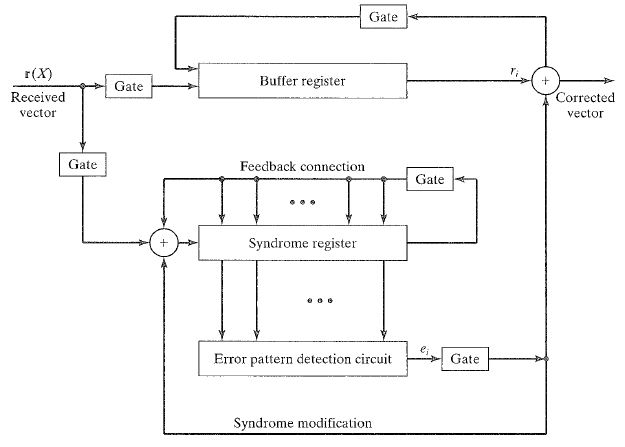
\includegraphics[width=0.7\linewidth]{./Picture/Meggitt_decoder}
\caption[The Meggitt decoder]{Meggitt decoder overview}
\label{fig:Meggitt_decoder}
\end{figure}

Figure \ref{fig:Meggitt_decoder_example} shows in more details how the syndrome register could be build together with the error pattern detection circuit.
The feedback in the syndrome register is depending on the general polynomial.
The number of bits in the syndrome is equal to the highest degree in g(X).
The non zero places in the general vector will get the feedback.
In this example the generator polynomial is $1+X+X^3$.
Therefore there will be feedback before 1 and X and the feedback is given by $X^3$.
The generator polynomial used in this project is: $g(X)=1+X^4+X^6+X^7+X^8$.
The feedback in the syndrome register will therefore happen before memory block 1, 5, 7 and 8. \fxnote{\textbf{See Figure \dots}}

\begin{figure}[htbp]
\centering
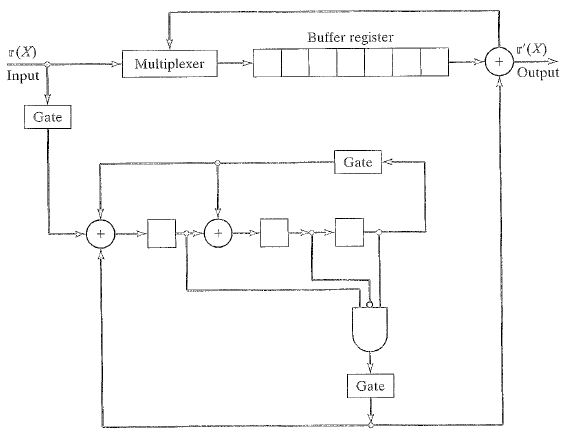
\includegraphics[width=0.7\linewidth]{./Picture/Meggitt_decoder_example}
\caption[Meggit Decoder example]{Meggitt decoder details}
\label{fig:Meggitt_decoder_example}
\end{figure}

The Meggitt decoder contains of 5 steps:
\begin{enumerate}
\item The received vector is shifted into the buffer register and syndrome register.
At this point the feedback from the error pattern circuit is not used.
\item The syndrome is check in the error pattern detection circuit.
If the syndrome is in the error pattern lookup table there is an error in the last bit in the buffer register and the error pattern detection circuit output will be 1.
If the syndrome don't match any error pattern it output will be 0.
\item The rightmost symbol in the buffer register is read out at the same time as the syndrome register is shifted once.
If an error has been detected it is feedback to he shifted syndrome register which modify the syndrome.
The error is also multiplied to the symbol which has been read out of the buffer. 
\item The new syndrome is match the new rightmost symbol in the buffer.
Step 2 and 3 is repeated.
\item The received vector is decoded symbol by symbol until the whole receive vector has been read out of the buffer register.
\end{enumerate}

\subsubsection{Meggitt decode example}
In this example the codeword $ c = [0 1 1 1 1 0 0 0 1 0 0 1 1 0 1] $ is used.
An error is made on bit 7 which mean $X^6$ is flipped.
The received vector is: $ r = [0 1 1 1 1 0 {\color{red}1} 0 1 0 0 1 1 0 1] $.
At first r(X) is shifted into the syndrome register.
The first 8 step is straight forward because where will be no feedback at the syndrome register is initialized with all zeroes at the beginning.
\begin{eqnarray*}
\textbf{shift no. \quad	input \qquad syndrome}\\
shift_1: \quad input = 1 \quad \Rightarrow \quad 10000000\\
shift_2: \quad input = 0 \quad \Rightarrow \quad 01000000\\
shift_3: \quad input = 1 \quad \Rightarrow \quad 10100000\\
shift_4: \quad input = 1 \quad \Rightarrow \quad 11010000\\
shift_5: \quad input = 0 \quad \Rightarrow \quad 01101000\\
shift_6: \quad input = 0 \quad \Rightarrow \quad 00110100\\
shift_7: \quad input = 1 \quad \Rightarrow \quad 10011010\\
shift_8: \quad input = 0 \quad \Rightarrow \quad 01001101
\end{eqnarray*}
The next 7 shift is it possible to get feedback.
The bit coloured light blue is the one which receive feedback. 
\begin{eqnarray*}
\textbf{shift no. \quad	input \quad old syn \qquad \quad new syn}\\
shift_9: \quad input = 1 \quad 010{\color{cyan}1}0{\color{cyan}11}01 \quad \Rightarrow \quad 00101101\\
shift_{10}: \quad input = 0 \quad 001{\color{cyan}0}1{\color{cyan}10}1 \quad \Rightarrow \quad 10011101\\
shift_{11}: \quad input = 1 \quad 100{\color{cyan}1}1{\color{cyan}10}1 \quad \Rightarrow \quad 01000101\\
shift_{12}: \quad input = 1 \quad 010{\color{cyan}0}0{\color{cyan}10}1 \quad \Rightarrow \quad 00101001\\
shift_{13}: \quad input = 1 \quad 001{\color{cyan}0}1{\color{cyan}00}1 \quad \Rightarrow \quad 00011111\\
shift_{14}: \quad input = 1 \quad 000{\color{cyan}1}1{\color{cyan}11}1 \quad \Rightarrow \quad 00000100\\
shift_{15}: \quad input = 0 \quad 000{\color{cyan}0}0{\color{cyan}10}0 \quad \Rightarrow \quad 00000010
\end{eqnarray*}
After shifted $r(X)$ into the syndrome register the syndrome has a 1 on the 7'th bit, which is the syndrome pattern matching the error pattern for $X^6$.
This bit was flipped in the received vector to introduce an error.
Another way to find the syndrome matching $ r(X) $ is to make the polynomial division as in Equation \ref{syndrom formular}. \fxnote{SKAL DETTE BEVISES?}

The $r(X)$ in the buffer match the $S(X)$ in the syndrome register, but what happens with $S(X)$ when the $r(X)$ is shifted in the buffer?
When $r(X)$ is cyclic right shifted it becomes $r^{(1)}(X)$ and has a cosponsoring $S^{(1)}(X)$.
This $S^{(1)}(X)$ can be found by multiply it with X and make a polynomial division with $g(X)$ as shown below.
\begin{eqnarray}
\label{S(X) after right shift}
S^{(1)}(X) = X \cdot S(X) \: mod \: g(X)
\end{eqnarray} 
The list of shifts below shows how the syndrome is changing when right shifting.
The input is no longer from $r(X)$ but is the error output, which is zero when no error has been detected in the last bit. 
Looking at shift 3 as an example of Equation \ref{S(X) after right shift}, the syndrome register contains $10001011 \Rightarrow 1+X^4+X^6+X^7$ before shifting.
When right shifting it becomes $X+X^5+X^7+X^8 = X \cdot S(X)$.
Finding $S^{(1)}(X)$ with the polynomial division of $g(X)$ gives $1+X+X^4+X^5+X^6 \Rightarrow 11001110$.
This $S^{(1)}(X)$ match the $r^{(1)}(X)$ which is in the buffer after the shift.
\begin{eqnarray*}
\textbf{shift no. \quad	input \quad old syn \qquad \quad new syn}\\
shift_1: \quad input = 0 \quad 00000010 \quad \Rightarrow \quad 00000001\\
shift_2: \quad input = 0 \quad 00000001 \quad \Rightarrow \quad 10001011\\
shift_3: \quad input = 0 \quad 10001011 \quad \Rightarrow \quad 11001110\\
shift_3: \quad input = 0 \quad 11001110 \quad \Rightarrow \quad 01100111\\
shift_4: \quad input = 0 \quad 01100111 \quad \Rightarrow \quad 10111000\\
shift_5: \quad input = 0 \quad 10111000 \quad \Rightarrow \quad 01011100\\
shift_6: \quad input = 0 \quad 01011100 \quad \Rightarrow \quad 00101110\\
shift_7: \quad input = 0 \quad 00101110 \quad \Rightarrow \quad 00010111\\
shift_8: \quad input = 1 \quad 00010111 \quad \Rightarrow \quad 00000000
\end{eqnarray*}
After shift 7 the syndrome match the error pattern for one error at the last bit.
After the 8'th bit the syndrome becomes an all zero vector, which indicates that there is no more errors in the buffer.

The only error that is interesting is the last error, therefore when correcting 1 error only the error pattern for error in the rightmost symbol is used.
In our example the error pattern will be $e(X) = [000000000000001]$.
When introducing 2 errors correcting the error pattern is extended to the one shown in list:\fxnote{INDSÆT LINK HER MAIKEN!}.

\begin{equation}
syndromeErrorPattern = 
\begin{bmatrix}
     0 &    0 &    0 &    1 &    0 &    1 &    1  &   1\\
     0 &    0 &    1 &    1 &    1 &    0 &    0  &   1\\
     0 &    1 &    0 &    0 &    1 &    0 &    1  &   1\\
     1 &    0 &    1 &    0 &    1 &    1 &    1  &   1\\
     0 &    1 &    1 &    1 &    0 &    0 &    0  &   0\\
     1 &    1 &    0 &    1 &    1 &    0 &    0  &   1\\
     1 &    0 &    0 &    1 &    1 &    1 &    0  &   0\\
     0 &    0 &    0 &    1 &    0 &    1 &    1  &   0\\
     0 &    0 &    0 &    1 &    0 &    1 &    0  &   1\\
     0 &    0 &    0 &    1 &    0 &    0 &    1  &   1\\
     0 &    0 &    0 &    1 &    1 &    1 &    1  &   1\\
     0 &    0 &    0 &    0 &    0 &    1 &    1  &   1\\
     0 &    0 &    1 &    1 &    0 &    1 &    1  &   1\\
     0 &    1 &    0 &    1 &    0 &    1 &    1  &   1\\
     1 &    0 &    0 &    1 &    0 &    1 &    1  &   1
\end{bmatrix}
\end{equation}

Even though the code is looking for 2 error it is still only errors on the rightmost bit in the buffer that are of interest.
Therefore the error pattern will contain all possible 2 errors where the one is fixed on the to the right.
To find the corresponding syndrome error pattern matching a specific error pattern the error pattern is divided with the general polynomial.
This is done for all the interesting error patterns and the syndromes used for matching in the error pattern detection circuit.
\end{document}
